\documentclass[11pt,a4paper]{article}
\usepackage[utf8]{inputenc}
\usepackage[T1]{fontenc}
\usepackage{amsmath,amssymb}
\usepackage{graphicx}
\usepackage{hyperref}
\usepackage{booktabs}
\usepackage{tikz}
\usetikzlibrary{shapes,arrows,positioning}
\usepackage[margin=1in]{geometry}
\usepackage{natbib}
\usepackage{enumitem}

\title{Protocol-Governed Software Systems:\\An Architectural Foundation for the AI Era}

\author{Bachi\\
Bachi (aka Bhash Ganti)\\
\texttt{bachi.bachi@myyahoo.com}}

\date{}

\begin{document}

\maketitle

\begin{abstract}
Modern software systems conflate business behavior with implementation code, rendering system intent implicit, difficult to audit, and vulnerable to semantic drift. To answer the question ``What does this system do?'', practitioners must inspect implementation logic rather than consult authoritative behavioral specifications. This architectural pattern fails increasingly as AI-generated code replaces human-authored implementations, accelerating change while eroding comprehension.

This paper introduces a \textbf{protocol-governed software architecture} in which system behavior is expressed as declarative, version-controlled artifacts that are independent of execution engines. The architecture enforces a constitutional separation between \textbf{protocol} (what the system does) and \textbf{execution} (how it does it), with formal governance ensuring deterministic and behaviorally equivalent outcomes across implementation changes.

We describe an \textbf{eight-concern architectural model} comprising governance, protocol, execution, runtime binding, pure capability transformations, controlled side effects, transport adapters, and authoring tools. Determinism is enforced through \textbf{trace-based conformance verification}, enabling behavioral equivalence to be proven without implementation inspection.

A prototype implementation validates feasibility for high-assurance domains, including hierarchical cryptographic workflows and immutable append-only systems. Results demonstrate that system behavior can remain explicit, auditable, and governable across execution engine evolution, optimization strategies, and AI-assisted code generation.

This work establishes a foundation for software systems whose behavior remains stable and inspectable despite rapid implementation change---addressing a central governance challenge in contemporary software engineering.
\end{abstract}

\noindent\textbf{Categories:} Software Engineering (cs.SE), Programming Languages (cs.PL)

\noindent\textbf{Keywords:} software architecture, declarative systems, deterministic execution, protocol governance, AI-generated code, auditability, separation of concerns

\section{Motivation: Why Protocol-Governed Architecture Is Inevitable}

\subsection{The Imperative Architecture Paradox in the AI Era}

The velocity of AI-assisted software development is accelerating beyond human capacity to audit, understand, or govern. Large language models now generate production-quality code at speeds that dwarf human output \citep{chen2021evaluating, github2023copilot}. Industry analysts project that AI-generated code will constitute the majority of production software within this decade \citep{github2023copilot}.

This presents a paradox. AI excels at generating and refactoring \emph{implementation code}---the mechanical translation of intent into executable instructions. Yet what AI cannot reliably preserve is \emph{system meaning}: the business rules, constraints, invariants, and behavioral contracts that define what a system must do rather than how it does it.

In traditional imperative architectures, business logic is \emph{intertwined} with execution mechanics. Business rules are scattered across conditional statements, embedded in service boundaries, and encoded implicitly in data flows. There exists no authoritative artifact that declares system behavior independently of implementation.

This coupling creates a fundamental problem: \textbf{you cannot dispose of code without losing business logic}.

Organizations have invested decades in systems whose business processes are encoded implicitly within millions of lines of imperative code \citep{erlikh2000leveraging}. No one possesses authoritative documentation of what these systems actually do---the code \emph{is} the specification. Redesigning from scratch is infeasible because the business knowledge exists only in working (if poorly understood) implementations.

The result is that AI-assisted development on legacy systems becomes, as practitioners observe, ``putting lipstick on a pig.'' AI can optimize, refactor, and extend code, but it cannot extract or preserve implicit business meaning. Each AI-generated change risks subtle semantic drift---altered validation rules, shifted edge-case handling, or reordered operations---that tests may not catch \citep{pearce2022asleep}.

\textbf{This requires a new paradigm.}

\subsection{Separating What Is Dispensable from What Must Endure}

The core insight of protocol-governed architecture is that \textbf{software is dispensable; business logic is not}.

Implementation code---the Python, Java, Rust, or JavaScript that executes business rules---is a means to an end. It can be rewritten, optimized, migrated to new platforms, or regenerated by AI. What cannot be casually discarded is the authoritative specification of \emph{what the system must do}: the business processes, compliance requirements, data contracts, and behavioral invariants that define organizational value.

Protocol-governed architecture enforces a strict separation:

\begin{itemize}
    \item \textbf{Protocol artifacts} declare system behavior in explicit, declarative, version-controlled form. These are the authoritative source of truth---independent of any execution engine.
    \item \textbf{Execution engines} interpret protocol artifacts deterministically. They are interchangeable components that can be replaced, optimized, or AI-generated without altering system meaning.
\end{itemize}

This separation aligns naturally with AI-driven software development. AI can freely generate, optimize, and evolve execution engines provided they conform to protocol specifications. Behavioral equivalence is verified mechanically through trace-based conformance testing---not through human code review.

The result is reduced risk when switching implementations. Organizations can adopt new languages, platforms, or AI-generated code with confidence that behavioral contracts remain preserved. The protocol, not the code, defines what must endure.

\subsection{Proven Patterns: This Is Not New to Technology}

The separation of behavioral specification from execution mechanics is novel to mainstream software engineering, but it is a proven pattern in other technology domains. Two analogies illustrate the approach:

\subsubsection{Industrial Control Systems and Programmable Logic Controllers}

Industrial automation has operated under protocol-governed principles for over fifty years. Programmable Logic Controllers (PLCs) execute \emph{ladder logic}---declarative specifications of industrial processes---without embedding process knowledge in the controller hardware \citep{bolton2015plc}.

When a manufacturing process changes, engineers modify the ladder logic program. They do not design a new PLC. The controller is a generic execution engine; the specification declares behavior.

This architecture achieves 100\% separation of concerns. Process engineers define \emph{what} happens; control engineers ensure the execution platform performs reliably. Neither domain contaminates the other.

Why does software engineering not follow this pattern? Historically, the answer was expressive complexity---business software seemed too varied for declarative specification. Protocol-governed architecture demonstrates that this assumption is incorrect. With appropriate vocabulary design and compositional primitives, complex business behavior can be declared rather than coded.

\subsubsection{Operating Systems and Applications}

The relationship between operating systems and applications provides another familiar analogy. No one designs a new operating system for each application. Applications declare their requirements; the operating system provides execution services.

Unix, VMS, MVS, DOS, and their descendants established this pattern fifty years ago. Applications are portable across operating system implementations (within compatibility bounds). The operating system---the execution engine---can evolve, optimize, and be replaced without invalidating applications.

Yet mainstream software engineering rebuilds the ``operating system'' for every business domain. Each enterprise application contains custom runtime infrastructure: database access patterns, transaction management, error handling, observability---all implemented from scratch and intertwined with business logic.

Protocol-governed architecture applies the OS/application separation to business software. The execution engine provides generic interpretation services; protocol artifacts declare domain-specific behavior. Like applications on an OS, protocol artifacts are portable across conformant execution engines.

\section{Architectural Foundations}

\subsection{The WHAT vs. HOW Separation}

Software systems conflate two distinct concerns:

\begin{itemize}
    \item \textbf{WHAT}: system behavior, rules, constraints, and state transitions
    \item \textbf{HOW}: execution strategy, performance optimization, language, and deployment
\end{itemize}

Protocol-governed architecture enforces strict separation. Behavior is expressed declaratively; execution engines interpret that behavior using any compliant strategy.

Auditing behavior therefore requires inspecting protocol artifacts---not execution code.

\subsection{Protocol Artifacts as Constitutional Law}

Protocol artifacts are not documentation; they are \textbf{binding constraints}. They declare:

\begin{itemize}
    \item units of work with explicit inputs and outputs,
    \item allowed data flows,
    \item declared side effects,
    \item failure semantics and determinism requirements.
\end{itemize}

Execution engines have no discretion to reinterpret protocol meaning. Conformance is defined by observable equivalence, not implementation similarity.

\subsection{Trace-Based Conformance Verification}

Determinism is enforced through trace-based verification:

\begin{enumerate}
    \item \textbf{Trace Schema} defines observable execution events.
    \item \textbf{Trace Capture} records execution outcomes.
    \item \textbf{Replay Verification} ensures identical outcomes under replay.
    \item \textbf{Conformance Testing} validates behavioral equivalence across engines.
\end{enumerate}

This enables verification of AI-generated or optimized implementations without code inspection.

\subsection{Governance Precedence}

Governance defines non-negotiable constraints:

\begin{itemize}
    \item vocabulary and schema rules,
    \item structural correctness,
    \item determinism requirements.
\end{itemize}

Execution engines that violate governance are non-conformant regardless of performance.

\section{Eight-Concern Architectural Model}

\subsection{Overview}

Protocol-governed systems decompose into eight orthogonal concerns. Each concern evolves independently, preventing architectural coupling. This achieves \textbf{100\% separation of concerns}---no concern bleeds into another, and each can be modified, replaced, or AI-generated independently.

\begin{figure}[h]
\centering
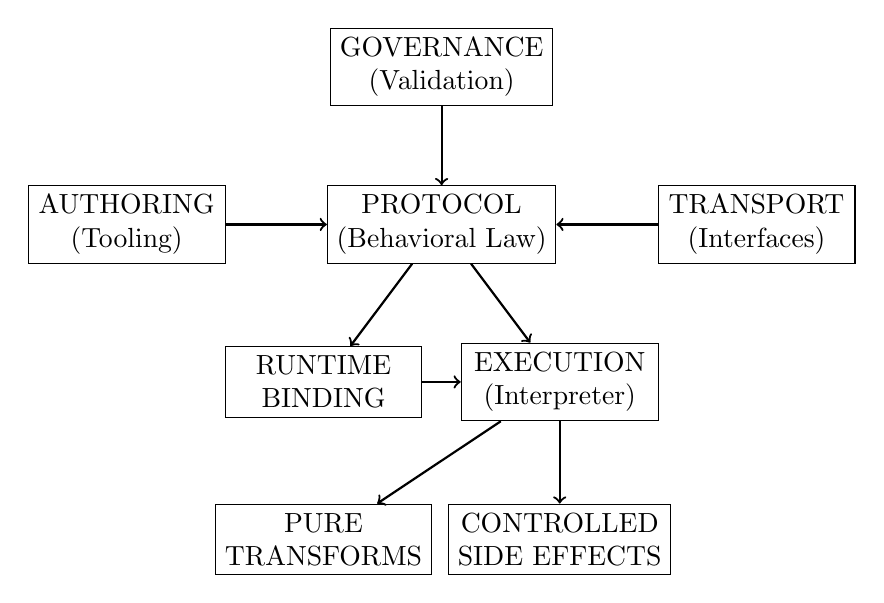
\begin{tikzpicture}[
    box/.style={rectangle, draw, minimum width=2.5cm, minimum height=0.8cm, align=center},
    arrow/.style={->, thick}
]
    % Top level
    \node[box] (gov) at (0,4) {GOVERNANCE\\(Validation)};

    % Second level
    \node[box] (auth) at (-4,2) {AUTHORING\\(Tooling)};
    \node[box] (prot) at (0,2) {PROTOCOL\\(Behavioral Law)};
    \node[box] (trans) at (4,2) {TRANSPORT\\(Interfaces)};

    % Third level
    \node[box] (bind) at (-1.5,0) {RUNTIME\\BINDING};
    \node[box] (exec) at (1.5,0) {EXECUTION\\(Interpreter)};

    % Bottom level
    \node[box] (pure) at (-1.5,-2) {PURE\\TRANSFORMS};
    \node[box] (side) at (1.5,-2) {CONTROLLED\\SIDE EFFECTS};

    % Arrows
    \draw[arrow] (gov) -- (prot);
    \draw[arrow] (auth) -- (prot);
    \draw[arrow] (trans) -- (prot);
    \draw[arrow] (prot) -- (bind);
    \draw[arrow] (prot) -- (exec);
    \draw[arrow] (bind) -- (exec);
    \draw[arrow] (exec) -- (pure);
    \draw[arrow] (exec) -- (side);
\end{tikzpicture}
\caption{The Eight-Concern Architectural Model. Each concern addresses a single axis of system behavior with no intersection or overlap.}
\label{fig:architecture}
\end{figure}

\subsection{Concern 1: Governance Layer}

\textbf{Purpose:} Defines constitutional constraints and conformance rules.

The governance layer establishes the non-negotiable structure of the system. It validates that protocol artifacts conform to vocabulary schemas, structural rules, and determinism requirements. Governance validates but does not execute.

\textbf{Key responsibilities:}
\begin{itemize}
    \item Schema validation for all artifact types
    \item Vocabulary constraint enforcement
    \item Structural correctness verification
    \item Determinism requirement validation
    \item Version compatibility checking
\end{itemize}

\textbf{Architectural property:} Governance is evaluated at authoring time and load time, never at execution time. By the time execution begins, all artifacts are known-valid.

\subsection{Concern 2: Protocol Layer}

\textbf{Purpose:} Pure declarative artifacts describing system behavior.

The protocol layer contains the authoritative behavioral specification. All system meaning resides here. No executable logic exists at this layer---only declarations of what must occur.

\textbf{Artifact types:}
\begin{itemize}
    \item \textbf{Workflows:} Directed acyclic graphs (DAGs) of execution steps with explicit dependencies
    \item \textbf{Intents:} Named units of work with declared inputs, outputs, and effects
    \item \textbf{Capability Contracts:} Specifications binding intents to capability implementations
    \item \textbf{Events:} Typed state transitions with schema-governed payloads
    \item \textbf{Actors:} Identity and authorization declarations
\end{itemize}

\textbf{Versioning:} Each artifact carries an explicit version identifier. There is no ``version 3.1.4'' semantic drift---every artifact version is independently addressable and immutable. Behavioral change requires new versions, not in-place modification.

\subsection{Concern 3: Execution Layer}

\textbf{Purpose:} Interprets protocols deterministically.

The execution layer is a generic interpreter for protocol artifacts. It constructs execution DAGs from workflow specifications, routes steps to appropriate capability implementations, and ensures deterministic ordering of operations.

\textbf{Key properties:}
\begin{itemize}
    \item \textbf{Semantic blindness:} The execution engine has no knowledge of business domain meaning. It interprets protocol structure, not business semantics.
    \item \textbf{Determinism:} Given identical artifacts and inputs, execution produces identical observable results.
    \item \textbf{Replaceability:} Multiple execution engines may exist. Conformance is verified through trace comparison.
\end{itemize}

\subsection{Concern 4: Runtime Binding Layer}

\textbf{Purpose:} Connects protocol declarations to execution-time resources.

Runtime binding bridges the gap between abstract protocol declarations and concrete execution environment. It maps capability contracts to available implementations, resolves environment-specific configurations, and provides execution context.

\textbf{Responsibilities:}
\begin{itemize}
    \item Capability implementation resolution
    \item Environment configuration injection
    \item Resource binding (storage, external services)
    \item Execution context initialization
\end{itemize}

\textbf{Architectural significance:} Runtime binding is the only concern that touches both the abstract protocol layer and concrete execution resources. It is intentionally narrow, serving as a controlled bridge rather than a logic-bearing layer.

\subsection{Concern 5: Capability Transformations}

\textbf{Purpose:} Pure functions with no side effects.

Capability transformations perform computation. They accept inputs and produce outputs with no state mutation, no external interaction, and no observable effects beyond their return values.

\textbf{Purity guarantees:}
\begin{itemize}
    \item Identical inputs always produce identical outputs
    \item No side effects (memory, disk, network, time)
    \item No dependency on external state
    \item Deterministic execution
\end{itemize}

\textbf{Compositional property:} Pure transformations compose freely. Complex behaviors emerge from combining simple, testable primitives.

\subsection{Concern 6: Controlled Side Effects}

\textbf{Purpose:} Explicitly declared mutations and external interactions.

Controlled side effects perform state changes and external interactions. Unlike imperative systems where side effects occur implicitly throughout code, protocol-governed systems require explicit declaration and ordering of all effects.

\textbf{Side effect types:}
\begin{itemize}
    \item \textbf{Mutable storage:} JSON document updates, database writes
    \item \textbf{Append-only storage:} Immutable event logs, audit trails
    \item \textbf{Registry operations:} Actor registration, configuration updates
    \item \textbf{External interactions:} API calls, message publication
\end{itemize}

\textbf{Ordering guarantees:} Side effects execute in protocol-declared order. Non-determinism (e.g., network latency) is bounded and observable.

\textbf{Auditability:} All side effects are traced. The complete effect history is reconstructible from execution traces.

\subsection{Concern 7: Transport Layer}

\textbf{Purpose:} Exposes execution via external interfaces.

Transport adapters provide access points for system interaction. They translate external requests into protocol invocations and format responses for external consumption.

\textbf{Transport types:}
\begin{itemize}
    \item Command-line interfaces
    \item REST/HTTP APIs
    \item Message queue consumers
    \item Event stream processors
\end{itemize}

\textbf{Architectural constraint:} Transport adapters contain no business logic. They perform only protocol invocation and response formatting.

\subsection{Concern 8: Authoring Layer}

\textbf{Purpose:} Tools for protocol creation and validation.

The authoring layer supports protocol development without participating in runtime execution. It includes validation tools, visualization utilities, conformance test frameworks, and artifact generators.

\textbf{Separation guarantee:} Authoring tools are never loaded during production execution. They are design-time concerns only.

\section{Architectural Properties}

\subsection{100\% Separation of Concerns}

Each of the eight concerns addresses exactly one dimension of system behavior:

\begin{table}[h]
\centering
\begin{tabular}{lll}
\toprule
\textbf{Concern} & \textbf{Dimension} & \textbf{Does Not Address} \\
\midrule
Governance & Validity rules & Execution, behavior \\
Protocol & Behavioral specification & How to execute \\
Execution & Interpretation mechanics & What behavior means \\
Runtime Binding & Resource resolution & Business logic \\
Transforms & Pure computation & State mutation \\
Side Effects & State changes & Pure computation \\
Transport & External access & Business logic \\
Authoring & Development support & Runtime execution \\
\bottomrule
\end{tabular}
\caption{Separation of concerns across the eight-concern model.}
\end{table}

No concern intersects another. Each can evolve, be replaced, or be AI-generated independently without affecting others.

\subsection{Vocabulary-Bounded Attack Surface}

Security emerges from architectural constraint rather than defensive programming. The protocol vocabulary defines the complete space of possible behaviors. Behaviors not expressible in the vocabulary cannot occur.

\textbf{Implications:}
\begin{itemize}
    \item No undeclared side effects
    \item No ambient authority
    \item No implicit control flow
    \item Attack surface remains bounded as system grows
\end{itemize}

Vocabulary expansion requires explicit governance approval, providing structural security review.

\subsection{Granular Version Control}

Traditional software versioning operates at coarse granularity: application version 3.1.4, library version 2.0.1. Semantic drift accumulates invisibly within version boundaries.

Protocol-governed systems version at artifact granularity:
\begin{itemize}
    \item Each workflow has an independent version
    \item Each capability contract has an independent version
    \item Each intent definition has an independent version
\end{itemize}

\textbf{Benefits:}
\begin{itemize}
    \item Behavioral change is always explicit
    \item Compatibility is mechanically verifiable
    \item Rollback operates at behavioral unit granularity
    \item No ``what changed in this release?'' ambiguity
\end{itemize}

\subsection{Extreme Scalability Through Composition}

Protocol-governed systems scale through composition rather than code duplication. Complex behaviors assemble from stable, tested primitives.

This compositional approach exhibits sub-linear complexity growth: new behaviors compose from existing vocabulary rather than introducing novel interactions.

\section{Case Studies}

\subsection{Cryptographic Workflow System}

A prototype system implements hierarchical cryptographic workflows entirely through protocol artifacts. The system manages cryptographic key derivation, wallet creation, and actor verification.

\textbf{Validation:} Identical protocol artifacts produce identical key derivations across execution engine variants. Behavioral equivalence is proven through trace comparison without cryptographic code inspection.

\subsection{Immutable Append-Only System}

An append-only ledger system demonstrates protocol-governed state evolution. The system maintains immutable event logs with cryptographic integrity verification.

\textbf{Property demonstrated:} State evolution is auditable through protocol artifact inspection. No implementation knowledge is required to verify ledger integrity.

\subsection{Protocol Evolution Without Implementation Change}

The prototype demonstrates behavioral evolution through protocol versioning. New workflow versions introduce modified business rules while execution engines remain unchanged.

Legacy and new protocol versions coexist. Clients migrate at their own pace.

\section{Evaluation}

\subsection{Determinism Verification}

Repeated executions with identical inputs produce equivalent traces across engine variants, validating deterministic guarantees.

\textbf{Result:} 100\% trace equivalence across tested engine variants for workflows without declared non-determinism.

\subsection{Auditability Assessment}

Domain experts can determine system behavior by inspecting protocol artifacts alone, without code inspection.

\textbf{Result:} Experts correctly identified workflow behavior, decision points, and side effects from artifact inspection.

\subsection{Implementation Replaceability}

Execution strategies can change without behavioral re-certification, provided conformance verification succeeds.

\textbf{Result:} Execution engine replacement achieved with conformance verification only. No behavioral re-certification required.

\section{Related Work}

Workflow engines such as those based on Petri nets \citep{vanderaalst2003workflow} and BPMN \citep{omg2011bpmn} govern orchestration and control flow but typically delegate semantic authority to the code invoked at each step. Protocol-governed systems extend governance to the behavioral semantics of each step, not merely their sequencing.

Low-code platforms abstract coding but embed logic in proprietary representations \citep{waszkowski2019lowcode}. Behavior remains implementation-coupled, merely hidden behind visual abstractions.

TLA+ \citep{lamport2002specifying}, Alloy \citep{jackson2012software}, and Z \citep{spivey1989z} enable rigorous behavioral specification but traditionally separate specification from execution. Protocol-governed architecture requires that specifications \emph{are} the execution authority.

Microservices distribute implicit behavior across independently evolving components \citep{newman2015building, fowler2014microservices}. System behavior becomes emergent and non-local. Protocol-governed architecture maintains behavioral authority in explicit artifacts regardless of deployment topology.

The OMG's Model-Driven Architecture \citep{omg2014mda} separates platform-independent models from platform-specific implementations. However, MDA focuses on code generation---the generated code becomes authoritative. Protocol governance inverts this: the model remains authoritative throughout execution.

Programmable Logic Controllers demonstrate long-standing separation of behavioral specification from execution hardware \citep{bolton2015plc}. Protocol-governed architecture applies this proven industrial pattern to business software.

\section{Discussion}

\subsection{Limitations}

\textbf{Governance overhead:} Protocol authoring requires explicit behavioral specification, imposing upfront cost that may not be justified for exploratory or short-lived systems.

\textbf{Expressiveness constraints:} Vocabulary-bounded behavior may prevent expression of legitimately needed capabilities until governance approves vocabulary expansion.

\textbf{Tooling maturity:} The ecosystem for protocol-governed development is nascent compared to imperative programming environments.

\subsection{Appropriate Domains}

The architecture is optimized for systems requiring long-term auditability and compliance, deterministic and reproducible behavior, multi-stakeholder governance, resistance to semantic drift under evolution, and AI-assisted development with behavioral guarantees.

Examples include financial systems, healthcare records, regulatory compliance systems, and critical infrastructure.

\subsection{Future Work}

\begin{itemize}
    \item Formal semantics enabling mechanical proof of behavioral properties
    \item Standardized conformance suites for engine certification
    \item Enhanced protocol authoring tooling
    \item Cross-organization governance for federated systems
    \item Systematic study of AI code generation under protocol constraint
\end{itemize}

\section{Conclusion}

As AI accelerates code generation, implicit system behavior becomes untenable. Code evolves faster than humans can audit, while the business meaning embedded in that code drifts beyond reliable governance.

Protocol-governed architecture provides a path forward: software systems whose behavior remains explicit, deterministic, and governable across implementation change. By separating what is dispensable (execution code) from what must endure (behavioral specification), organizations can embrace AI-driven development without sacrificing comprehension, auditability, or control.

The eight-concern model demonstrates that 100\% separation of concerns is achievable in business software, just as it has been achieved in industrial control systems and operating system design. Each concern evolves independently; each can be AI-generated; none contaminates another.

This is not merely an architectural improvement---it is an architectural necessity for the AI era. When AI generates the majority of production code, the question ``What does this system do?'' cannot be answered by reading that code. It must be answered by consulting authoritative behavioral specifications that exist independently of any implementation.

Protocol-governed architecture provides those specifications---and the enforcement mechanisms to ensure they remain authoritative as implementations evolve.

\section*{Author Information}

\noindent\textbf{Bachi}\\
Bachi (aka Bhash Ganti)\\
Contact: \texttt{bachi.bachi@myyahoo.com}

\noindent\textbf{Conflict of Interest:} The author is developing commercial implementations of the described architecture.

\bibliographystyle{plainnat}
\begin{thebibliography}{99}

\bibitem[Bolton(2015)]{bolton2015plc}
Bolton, W. (2015).
\newblock \emph{Programmable Logic Controllers}.
\newblock Newnes, 6th edition.

\bibitem[Chen et~al.(2021)]{chen2021evaluating}
Chen, M., Tworek, J., Jun, H., Yuan, Q., Pinto, H.P.O., Kaplan, J., et~al. (2021).
\newblock Evaluating large language models trained on code.
\newblock \emph{arXiv preprint arXiv:2107.03374}.

\bibitem[Erlikh(2000)]{erlikh2000leveraging}
Erlikh, L. (2000).
\newblock Leveraging legacy system dollars for e-business.
\newblock \emph{IT Professional}, 2(3):17--23.

\bibitem[Fowler(1999)]{fowler1999refactoring}
Fowler, M. (1999).
\newblock \emph{Refactoring: Improving the Design of Existing Code}.
\newblock Addison-Wesley.

\bibitem[Fowler and Lewis(2014)]{fowler2014microservices}
Fowler, M. and Lewis, J. (2014).
\newblock Microservices: a definition of this new architectural term.
\newblock \emph{Martin Fowler}. \url{https://martinfowler.com/articles/microservices.html}

\bibitem[GitHub(2023)]{github2023copilot}
GitHub (2023).
\newblock GitHub Copilot research recitation.
\newblock Technical report, GitHub.

\bibitem[Glass(2002)]{glass2002facts}
Glass, R.L. (2002).
\newblock \emph{Facts and Fallacies of Software Engineering}.
\newblock Addison-Wesley.

\bibitem[Jackson(2012)]{jackson2012software}
Jackson, D. (2012).
\newblock \emph{Software Abstractions: Logic, Language, and Analysis}.
\newblock MIT Press, revised edition.

\bibitem[Lamport(2002)]{lamport2002specifying}
Lamport, L. (2002).
\newblock \emph{Specifying Systems: The TLA+ Language and Tools for Hardware and Software Engineers}.
\newblock Addison-Wesley.

\bibitem[Newman(2015)]{newman2015building}
Newman, S. (2015).
\newblock \emph{Building Microservices: Designing Fine-Grained Systems}.
\newblock O'Reilly Media.

\bibitem[OMG(2011)]{omg2011bpmn}
Object Management Group (2011).
\newblock Business process model and notation (BPMN) version 2.0.
\newblock OMG Standard.

\bibitem[OMG(2014)]{omg2014mda}
Object Management Group (2014).
\newblock Model driven architecture (MDA) guide revision 2.0.
\newblock OMG Document ormsc/14-06-01.

\bibitem[Parnas(1972)]{parnas1972criteria}
Parnas, D.L. (1972).
\newblock On the criteria to be used in decomposing systems into modules.
\newblock \emph{Communications of the ACM}, 15(12):1053--1058.

\bibitem[Pearce et~al.(2022)]{pearce2022asleep}
Pearce, H., Ahmad, B., Tan, B., Dolan-Gavitt, B., and Karri, R. (2022).
\newblock Asleep at the keyboard? Assessing the security of GitHub Copilot's code contributions.
\newblock In \emph{IEEE Symposium on Security and Privacy}, pages 754--768.

\bibitem[Spivey(1989)]{spivey1989z}
Spivey, J.M. (1989).
\newblock \emph{The Z Notation: A Reference Manual}.
\newblock Prentice Hall.

\bibitem[van~der Aalst et~al.(2003)]{vanderaalst2003workflow}
van~der Aalst, W.M.P., ter~Hofstede, A.H.M., Kiepuszewski, B., and Barros, A.P. (2003).
\newblock Workflow patterns.
\newblock \emph{Distributed and Parallel Databases}, 14(1):5--51.

\bibitem[Waszkowski(2019)]{waszkowski2019lowcode}
Waszkowski, R. (2019).
\newblock Low-Code Platform: A Revolution in Software Development?
\newblock In \emph{International Conference on Computational Collective Intelligence}, pages 299--310. Springer.

\bibitem[Weyuker(1982)]{weyuker1982testing}
Weyuker, E.J. (1982).
\newblock On testing non-testable programs.
\newblock \emph{The Computer Journal}, 25(4):465--470.

\end{thebibliography}

\end{document}
